\documentclass{beamer}
%
% Choose how your presentation looks.
%
% For more themes, color themes and font themes, see:
% http://deic.uab.es/~iblanes/beamer_gallery/index_by_theme.html
%
\usetheme{Ilmenau}      % or try Darmstadt, Madrid, Warsaw, ...
\usecolortheme{seahorse} % or try albatross, beaver, crane, ...
\usefonttheme{default}  % or try serif, structurebold, ...
\setbeamertemplate{navigation symbols}{}
\setbeamertemplate{caption}[numbered]
\usepackage{tikz}
\usepackage{pgfplots}
\usepackage{pgf}
\usepackage{units}
\usepackage{graphicx}
\usepackage{caption}
\usepackage[mode=buildnew]{standalone}% requires -shell-escape
\usepackage{amsmath}

\usepackage[english]{babel}
\usepackage[utf8x]{inputenc}
\setbeamertemplate{footline}[frame number]

\title{Building an end-to-end speech recognizer}
\author{Moritz Wolter}

\date{01.02.2017}

\begin{document}
\begin{frame}
  \titlepage
\end{frame}


% Uncomment these lines for an automatically generated outline.
\begin{frame}{Outline}
  \tableofcontents
\end{frame}

\section{Introduction}
\begin{frame}{The problem}
	\begin{itemize}
		\item What is being said? 
		\item What is interesting?
		\item What model architecture?
		\item Which hyper-parameters?
		\item How to ensure generalization?
	\end{itemize}
\end{frame}

\subsection{Listen Attend and Spell}
\begin{frame}{Long Short Term Memory}
	\begin{figure}
		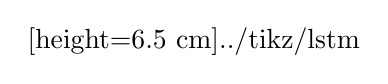
\begin{tikzpicture}
		    \node[anchor=south west,inner sep=0] at (0,0) {\includestandalone[height=6.5 cm]{../tikz/lstm}};
		    %\draw[red,ultra thick,rounded corners] (0.0,0.0) rectangle (5.0,2.5);
		\end{tikzpicture}
		\caption{LSTM cell architecture visualization.}
	\end{figure}
\end{frame}


\begin{frame}{The LAS-Architecture}
	\begin{figure}
		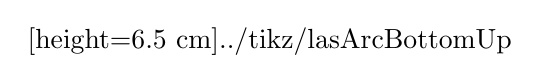
\begin{tikzpicture}
		    \node[anchor=south west,inner sep=0] at (0,0) {\includestandalone[height=6.5 cm]{../tikz/lasArcBottomUp}};
		    %\draw[red,ultra thick,rounded corners] (0.0,0.0) rectangle (5.0,2.5);
		\end{tikzpicture}
		\caption{Listener and speller.}
	\end{figure}
\end{frame}

\begin{frame}{The LAS-Equations}
Attend and spell cell computations:
\begin{align}
	 \mathbf{s}_i &= \text{RNN}(\mathbf{s}_{i-1}, \mathbf{y}_{i-1}, \mathbf{c}_{i-1}), \\
	 \mathbf{c}_i &= \text{AttentionContext}(\mathbf{s}_i,\mathbf{H}), \\
	  P(\mathbf{y}_i|\mathbf{x}, \mathbf{y}_{<i}) &= \text{CharacterDistribution}(\mathbf{s}_i,\textbf{c}_i).
\end{align}

AttentionContext computations:
\begin{align}
	e_{i,u} = \phi(\mathbf{s}_i)^T \psi(\mathbf{h_u}), \\
	\alpha_{i,u} = \frac{ \exp(e_{i,u})}{ \sum\limits_{u} \exp(e_{i,u})}, \\
	\label{eq:alphas}
	\mathbf{c}_i = \sum\limits_{u} \alpha_{i,u} \mathbf{h}_u.
\end{align}
\end{frame}


\section{Methodology}
\begin{frame}{Used methods}
	\begin{itemize}
		\item Object oriented programming, python.
			\begin{itemize}
				\item data encapsulation, partly replaced by \texttt{tf.variable\_scope}("...").
				\item code structure and re-usability.
			\end{itemize}
		\item Shape invariants, tensorflow.
			\begin{itemize}
				\item Programmer must explicitly state changing dimensions in loop.
				\item Makes code easier to read, and prevents bugs.
			\end{itemize}
		\item Code quality, pylint.
			\begin{itemize}
				\item if the python foundation' style guide is being followed. 
				\item looks for errors in the code.
			\end{itemize}
		\item Version control, git.
	\end{itemize}
\end{frame}

\section{Implementation}
\begin{frame}{Attend and spell cell layout}
	\begin{figure}
	\includestandalone[height=6.5 cm]{../tikz/asCellType1}
	\caption{Attend and spell cell flow chart.}
	\end{figure}
\end{frame}

\begin{frame}[fragile]
\frametitle{Decoding loop logic}
\begin{block}{body loop logic}
	\begin{semiverbatim}
	while keep_working:
	  not_done_count = reduce_sum( logical_not( d ))
	  done = equal(not_done_count, 0)
	  stop = logical_or(done, greater(time, max_steps))
	  keep_working = logical_not(stop)
	\end{semiverbatim}
\end{block}
\begin{block}{setting the sequence length}
	\begin{semiverbatim}
	  decoded = decode(logits)
	  mask = tf.equal(decoded, <eos>)
	  time_vec = ones(self.batch_size)*(time+1)
	  sequence_lengths = select(d,
	                            logits_sequence_length,
	                            time_vec)
	  d = logical_or(mask, d)
	\end{semiverbatim}
\end{block}
\end{frame}

\begin{frame}{Dropout}
	\begin{figure}
		\includestandalone[height=6.5 cm]{../tikz/las_dropout}
		\caption{Input dropout - light red. Hidden dropout - dark red.}
	\end{figure}
\end{frame}

\section{Results}
\begin{frame}{The Listener with CTC}
	\begin{figure}
		\includestandalone[width=0.49\textwidth]{../tikz/CTC_Listener_plot_e10_loss}
		\includestandalone[width=0.49\textwidth]{../tikz/CTC_Listener_plot_e10_error}
		\caption{Listener with attached CTC.}
	\end{figure}
\end{frame}


\subsection{Custom attention}

\begin{frame}{Greedy Decoding}
	\begin{figure}
	\includestandalone[width=0.49\linewidth]{../tikz/LAS_no_reg_e40_p07_loss}
	\includestandalone[width=0.49\linewidth]{../tikz/LAS_no_reg_e40_p07_error}
	\caption{The training progress shown for the full las architecture with greedy decoding, over 40 epochs, network output reuse probability 0.7 and input noise standard deviation 0.65 .}
	\label{fig:lasGreedy}
	\end{figure}
\end{frame}

\begin{frame}{Alignment plots}
	\begin{figure}
	\centering
	\includestandalone[width=0.49\linewidth]{../tikz/alpha}
	\includestandalone[width=0.42\linewidth]{../tikz/align}
	\caption{Plot of the alignment vectors computed by the network for all 45 labels assigned to timit utterance \texttt{fmld0\_sx295} (left), and alignments assigned by a human listener (right).}
	\label{fig:fullAttention}
	\end{figure}
\end{frame}

\begin{frame}{Alignment plots}
	\begin{block}{Target labels}
		\begin{semiverbatim}
		<sos>  sil  ih  f  sil  k  eh  r  l  sil  k  ah  m  z
		       sil  t  ah  m  aa  r  ah  hh  ae  v  er  r  ey
		       n  jh  f  er  m  iy  dx  iy  ng  ih  
		       sil  t  uw  sil
		<eos>
		\end{semiverbatim}
	\end{block}

	\begin{figure}
	\centering
	\includestandalone[height=0.26\linewidth]{../tikz/alphaZoom}
	\includestandalone[height=0.26\linewidth]{../tikz/alphaZoom2}
	\includestandalone[height=0.26\linewidth]{../tikz/alphaZoom3}
	\caption{Attention weights $\alpha$ and network output.}
	\label{fig:attention3}
	\end{figure}
\end{frame}

\begin{frame}
	\begin{figure}
	\centering
	\includestandalone[width=0.24\linewidth]{../tikz/LAS_no_reg_e10_p02_loss}
	\includestandalone[width=0.24\linewidth]{../tikz/LAS_no_reg_e10_p02_error}
	\includestandalone[width=0.24\linewidth]{../tikz/LAS_no_reg_e10_p04_loss}
	\includestandalone[width=0.24\linewidth]{../tikz/LAS_no_reg_e10_p04_error}
	\includestandalone[width=0.24\linewidth]{../tikz/LAS_no_reg_e10_p06_loss}
	\includestandalone[width=0.24\linewidth]{../tikz/LAS_no_reg_e10_p06_error}
	\includestandalone[width=0.24\linewidth]{../tikz/LAS_no_reg_e10_p08_loss}
	\includestandalone[width=0.24\linewidth]{../tikz/LAS_no_reg_e10_p08_error}
	\caption{Repetitions of the same experiment with increasing network output reuse probabilities $0.2, 0.4, 0.6, 0.8$, one experiment per row.}
	\label{fig:lasGreedy2468}
	\end{figure}
\end{frame}

\begin{frame}{Dropout las with beam search}
	\begin{figure}
	\includestandalone[width=0.49\textwidth]{../tikz/LAS_dropout0805_in00_p06_e120_double_loss}
	\includestandalone[width=0.49\textwidth]{../tikz/LAS_dropout0805_in00_p06_e120_double_error}
	\caption{Dropout las results.}
	\end{figure}
\end{frame}


\begin{frame}{Default attention}
TODO
\end{frame}

\begin{frame}{Conclusion}
TODO
\end{frame}


\section{Questions}
\begin{frame}{Questions}
	Thank's for your attention. Questions? \\
	Now, or later \texttt{moritz@wolter.tech}.
\end{frame}


\end{document}
